\documentclass[conference]{IEEEtran}
\IEEEoverridecommandlockouts
% The preceding line is only needed to identify funding in the first footnote. If that is unneeded, please comment it out.
\usepackage{cite}
\usepackage{amsmath,amssymb,amsfonts}
\usepackage{algorithmic}
\usepackage{graphicx}
\usepackage{textcomp}
\usepackage{xcolor}
\def\BibTeX{{\rm B\kern-.05em{\sc i\kern-.025em b}\kern-.08em
    T\kern-.1667em\lower.7ex\hbox{E}\kern-.125emX}}


\begin{document}

\title{Aided Navigation for Loosely-coupled INS/GNSS Sensor Fusion and Ideal IMU/Visual Simulation\\
% {\footnotesize \textsuperscript{*}Note: Sub-titles are not captured in Xplore and
% should not be used}
% \thanks{Identify applicable funding agency here. If none, delete this.}
}

\author{\IEEEauthorblockN{\textsuperscript{} Yang Qiyu}
% \IEEEauthorblockA{\textit{Student ID:122413910077} \\
Student ID:122413910077\\
% Shanghai Jiao Tong University
\textit{Shanghai Jiao Tong University}\\
% }

\and
\IEEEauthorblockN{\textsuperscript{} Liu Zhaohong}
% \IEEEauthorblockA{\textit{Student ID:122413910077} \\
Student ID:122413910061\\
% Shanghai Jiao Tong University
\textit{Shanghai Jiao Tong University}\\
% }

\and
\IEEEauthorblockN{\textsuperscript{} Zhang Yuxuan}
% \IEEEauthorblockA{\textit{Student ID:122413910077} \\
Student ID:122413910080\\
% Shanghai Jiao Tong University
\textit{Shanghai Jiao Tong University}\\

}

\maketitle

\begin{abstract}
GNSS technology has made navigation ubiquitous and has led to consumers salivating at the idea of importing this capability everywhere. Unfortunately, GNSS is not that much reliable in some places for various kinds of interference. This project will simulate an ideal IMU measurement and reference trajectory. After that, project will do fusion of an Inertial Navigation System (INS) and GNSS position information in an automotive application, via scripts generated by the app Nav Sensor Recorder, meaning to explain state of the art methods of modern aided navigation and multi-sensor localization.
This article also provides some basic localization practice using visual SLAM method,
especially the ORB-SLAM2 project.

\end{abstract}

\begin{IEEEkeywords}
IMU, INS, GNSS, Visual, Simulation, Multi-sensor, Fusion
\end{IEEEkeywords}

\section{Introduction}
As early as the 1960s, there were science fiction films and TV works depicting the autonomous navigation of mobile agents: intelligent robots that are able to travel freely in indoors such as in offices, factories, shopping malls, and hospitals and help people in work, production, play, and study. In these scenarios, autonomous navigation ability is the basic and one of the most important functions of mobile agents.
Autonomous indoor navigation of mobile agents refers to the abilities of autonomous localization and map construction in dynamic scenes This technology is based on the collection, analysis, and perception of environmental information, and carries out real-time localization and route planning by constructing a map. Using the data acquired by sensors to perceive the environment is the key technique related to mobile agent navigation. Historically, various sensors have been adopted for mobile agent navigation, such as cameras light detection and ranging (LiDAR) inertial measurement units (IMU) ultra-wide band (UWB) Wi-Fi Bluetooth ZigBee infrared ultrasonic, etc. According to the different principles and usages of these sensors, some scholars divided autonomous navigation into two categories: single-sensor navigation methods and multi-sensor fusion navigation methods.


In the single sensor navigation methods, the agents decide their own navigation states in the environment depending on a single sensor, among which cameras and LiDAR are widely used. A single sensor has specific advantages and limitations in navigation: for example, the visual sensor has the advantages of low price and various mature algorithms provided by researchers. However, the vision perception accuracies are easily influenced by the environments’ changes in illumination. 

Correspondingly, LiDAR data have the advantage of high frequency. However, LiDAR data’s resolution usually requires improvement and the content information is not intuitively presented in it. Compared to single-sensor agent navigation, multi-sensor fusion methods improve the localization accuracy and robustness in the task of navigation by collecting and fusing the environmental information from different types of sensors. In recent years, research on multi-sensor fusion methods for agent navigation has become an important trend.

The goal of this project is to realize and explain state of the art methods of modern aided navigation and multi-sensor localization. The software part in this project is written in Matlab for the sake of simplicity. Nevertheless, principal architecture of the sensor fusion software tries to ensure simple transferability to industrial software projects.

% \begin{table}[htbp]
% \caption{Speeds From Different Orbital Heightss}
% \begin{center}
% \begin{tabular}{|c|c|c|c|}
% \hline
% \multicolumn{1}{|c|}{} & \multicolumn{1}{c|}{GEO} & \multicolumn{1}{c|}{MEO} & \multicolumn{1}{c|}{LEO} \\
% \hline
% Distance from Earth &   35,786 Km &   8,000 Km &   550 Km\\
% Latency &   476 msec &   106.7 msec Km &  7.32 msec\\
% Data rate &   1.5 Mb/s &  2.1 Mb/s  &   150 Mb/s\\

% \hline
% % \multicolumn{4}{l}{$^{\mathrm{a}}$Sample of a Table footnote.}
% \end{tabular}
% \label{tab1}
% \end{center}
% \end{table}



% \begin{figure}[htbp]
%     \centerline{\includegraphics[width=1.0\columnwidth]{LEO1}}
%     \caption{Comparison of coverage of GEO, MEO and LEO satellites}
% \end{figure}



\section{Simulation of ideal IMU measurements and reference trajectory}

In this part, we will generate ideal IMU measurements from position and orientation timeseries provided by a vehicle simulator or measured by some navigation system in a field test. IMU data, generated by the provided software, allows to reconstruct reference trajectory by means of inertial navigation approach almost exactly.

\subsection{Principles of inertial navigation}

Accelerometers and gyroscopes are usually called inertial sensors. An accelerometer is a sensor that measures one or more projections of a specific force acting on a body. A gyroscope is a device for measuring projections of an angular rate of the body relatively to some inertial coordinate frame. Nowadays the abovementioned sensors are usually rigidly attached to the moving object which is why the measured values present the projections onto a body-fixed coordinate frame.

The core idea of inertial navigation consists in determining position and orientation of a moving object by means of integrating numerically differential equations of motion of a point mass in the neighborhood of Earth. Angular rate and specific force present inputs to the dynamic system and need to be measured by onboard inertial sensors. 

Additionally, initial position, velocity, and orientation are required to be known.

\subsection{Ideal IMU data}

Inertial navigation is a powerful tool for position, velocity, and orientation estimation. Its advantages are:

\begin{itemize}
  \item Availability of output at high rates
  \item No dependency to external signals, such as signals of GNSS
  \item Smoothness of output signals
  \item High level of robustness
\end{itemize}

However, in practice inertial navigation has some limitations. Due to presence of instrumental errors, such as offsets and noise, coordinates, provided by an inertial navigation system (INS) start to diverge from the true user location. For most modern MEMS inertial sensors divergence rate appears high and resembles “unbounded drift”. Nevertheless, IMU instrumental errors are not the only factor that contributes to error growth. Another important factor is accuracy of the numerical method employed to integrate INS ordinary differential equation. Even with the best available sensors, such as ring-laser gyroscopes, INS would “drift” relatively fast if the simplest 1st order Euler method was used for integration.

From the perspective of inertial navigation, IMU measurements would be ideal if they allowed to reconstruct vehicle’s trajectory and orientation perfectly. At this place it is important to add that this should be fulfilled only when sufficiently accurate numerical method is used and when integration step is small enough.

\subsection{Simulation Procedure}
Motion of a point mass in the neighborhood of Earth can be modeled by the ordinary differential equation given below. This equation and its derivation can be derived below:

\begin{equation}
\begin{array}{l}  
\dot X_{e} = V_{e} \\
\dot V_{e} = -2[\omega_{ie} \times]V_{e}+g_{e}(X_{e})+C_{es}(\breve q_{es})f_{s} \\
\dot{\breve{q}}_{es}  = 0.5(\breve q_{es}*\breve \omega_{is}-\breve \omega_{ie}*\breve q_{es})
\end{array} 
\end{equation}

The equations (1) can be used to express specific force and angular rate in terms of position, orientation, and their derivatives. Rearranging (1) yields:

\begin{equation}
\begin{array}{l}
\dot f_{s} = C_{es}^{-1}\breve q_{es}^{-1}(2[\omega_{ie} \times]V_{e}-g_{e}(X_{e})+\dot V_{e}) \\
\breve \omega_{is} = \breve q_{es}^{-1}(2\dot{\breve{q}}_{es}+\breve\omega_{ie}*\breve q_{es})
\end{array} 
\end{equation}

% \begin{figure}[htbp]
%     \centerline{\includegraphics[width=1.0\columnwidth]{iort.png}}
%     \caption{Comparison of coverage of GEO, MEO and LEO satellites}
% \end{figure}

Consider now timeseries $X_{e}(t_{k})$ and $\breve q_{e}(t_{k})$ are provided by some vehicle simulator (for example, X-Plane flight simulator) or measured by a navigation system in a test.

Then the following procedure can be employed to simulate ideal IMU measurements and a reference trajectory that corresponds to the measurements:

1.Downsample the timeseries $X_{e}(t_{k})$ and $\breve q_{e}(t_{k})$.

2.Derive Euler angles timeseries $\varphi(t_{k})$, $\upsilon(t_{k})$, $\psi(t_{k})$and $\breve q_{e}(t_{k})$ from the quaternion timeseries , unwrap range rollovers, if necessary.

3.Do spline interpolation of the position and Euler angles timeseries. Choose at least the third order spline.

4.Choose desired time grid $\tau$, $i = 1...N$. Any IMU data frequency is possible.

5.Differentiate position spline $x_e^{sp}$ two times to obtain velocity spline $\dot v_e^{sp}$ and acceleration spline .

6.Differentiate Euler angles splines $\varphi^{sp}$, $\upsilon^{sp}$, $\psi^{sp}$ to get the splines $\dot \varphi^{sp}$, $ \dot\upsilon^{sp}$, $\dot \psi^{sp}$

7.Evaluate the splines $x_e^{sp}$, $v_e^{sp}$, $\varphi^{sp}$, $\upsilon^{sp}$, $\psi^{sp}$at times $\tau_i$. This will yield reference position, velocity, and orientation.

8.Evaluate the splines $\dot x_e^{sp}$, $\dot v_e^{sp}$, $\dot \varphi^{sp}$, $\dot \upsilon^{sp}$, $\dot \psi^{sp}$at times $\tau_i$. This will yield auxiliary value.

9.Derive $\dot{\breve q}_{es}(\tau_i)$ form the reference Euler angles and their derivatives obtained in the steps 7 and 8. 

10.Use the equation (2) to compute $f_s(\tau_i)$ and $\breve{\omega}_s(\tau_i)$. Needed inputs: reference position, velocity, and orientation from the step 7, $\dot{v}_e(\tau_i)$ from the step 8, $\dot{\breve q}_{es}(\tau_i)$ from the step 9.

\subsection{Simlation Outcome}

Implementing the simulation procedure presented in the above Section. By default, the script simulates ideal IMU measurements at 100Hz. Figures 5-7 show deviations from reference of position, velocity, and orientation computed from the simulated IMU measurements by means of numerical integration of the differential equation (1) using Heun’s $2^{nd}$ order method. Orientation errors are of magnitude $10^{-5}$ [rad], velocity errors are on centimeter per second level, position errors get close to 15 meters.

Next, Figures 8-10 show INS errors for IMU data simulated at 50Hz rate. Note that each time when sensor rate gets 2 times lower, INS errors become exactly factor 4 larger. This effect is due to accuracy of the Heun’s method, which is a second order method. It means that decreasing/increasing integration step linearly should result into accuracy improving/degrading quadratically.

The observed effect serves as an evidence of IMU data being “ideal”, because residual INS errors can be explained by numerical effects. Choice of smaller step size and employment of more accurate integration method will mitigate inevitable error accumulation considerably.

\begin{figure}[htbp]
    \centerline{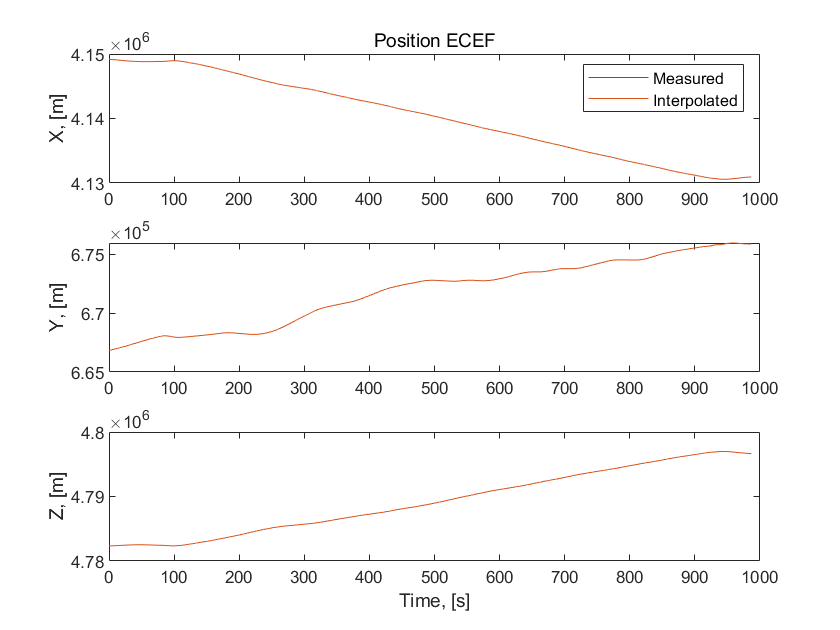
\includegraphics[width=1.0\columnwidth]{fig1.png}}
    \caption{Position ECEF}
\end{figure}

\begin{figure}[htbp]
    \centerline{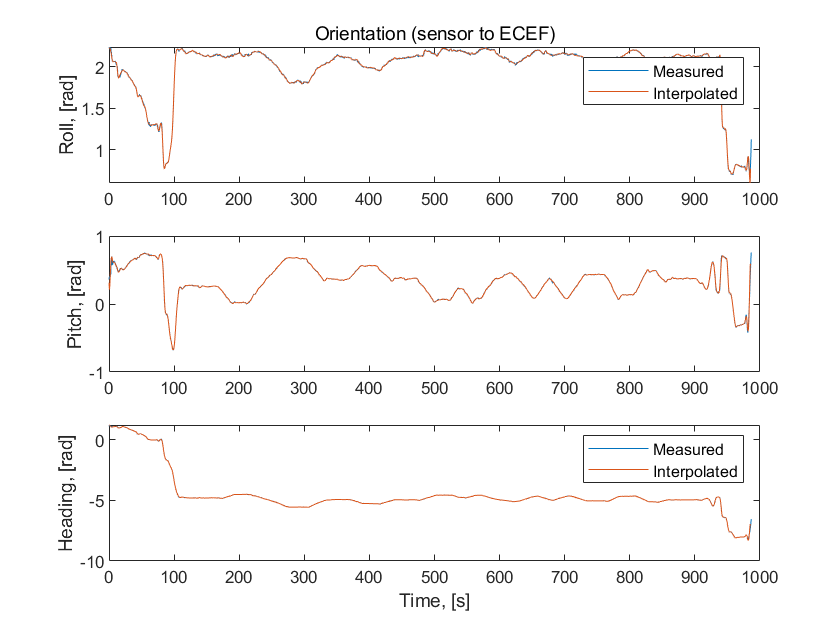
\includegraphics[width=1.0\columnwidth]{fig2.png}}
    \caption{Orientation(sensor to ECEF)}
\end{figure}

\begin{figure}[htbp]
    \centerline{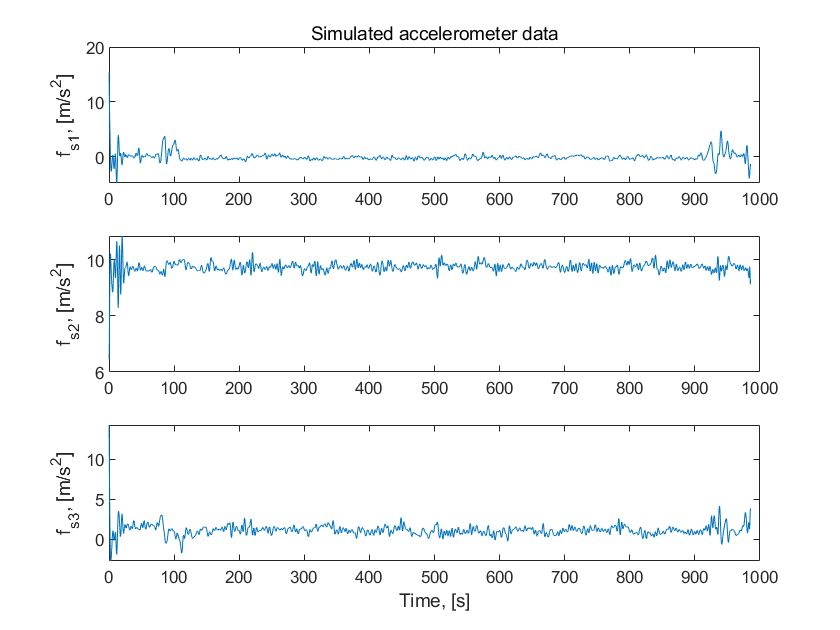
\includegraphics[width=1.0\columnwidth]{fig3.png}}
    \caption{Simulated accelerometer data}
\end{figure}

\begin{figure}[htbp]
    \centerline{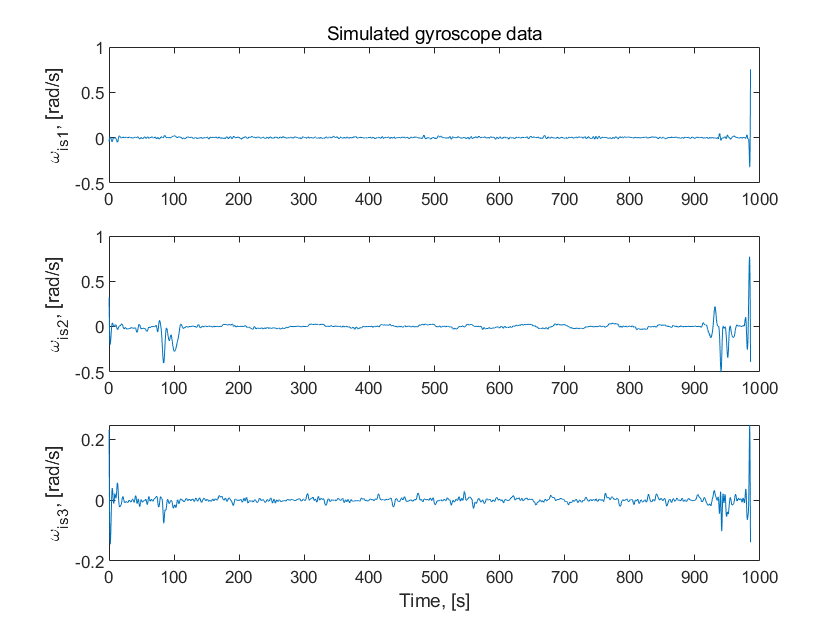
\includegraphics[width=1.0\columnwidth]{fig4.png}}
    \caption{Simulated gyroscope data}
\end{figure}

\begin{figure}[htbp]
    \centerline{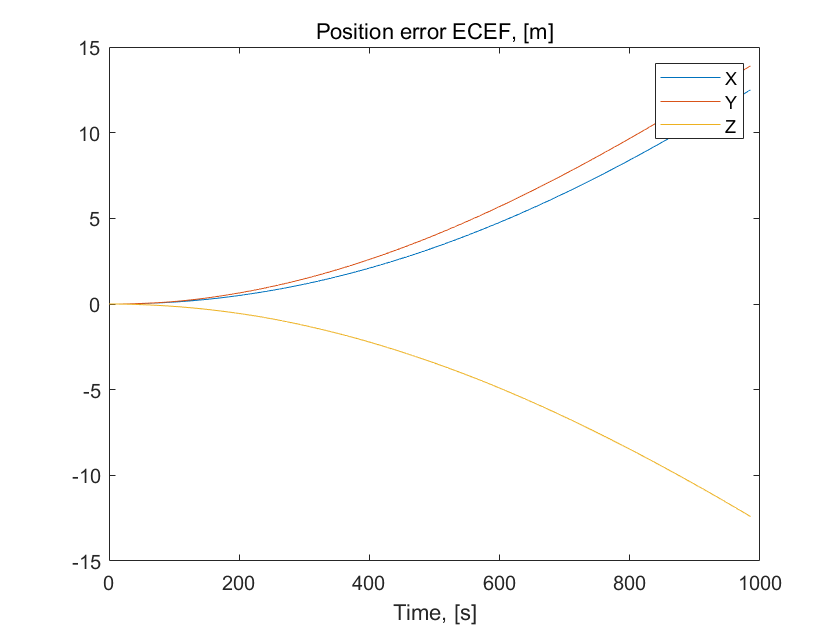
\includegraphics[width=1.0\columnwidth]{fig5.png}}
    \caption{Position error ECEF - 100Hz}
\end{figure}

\begin{figure}[htbp]
    \centerline{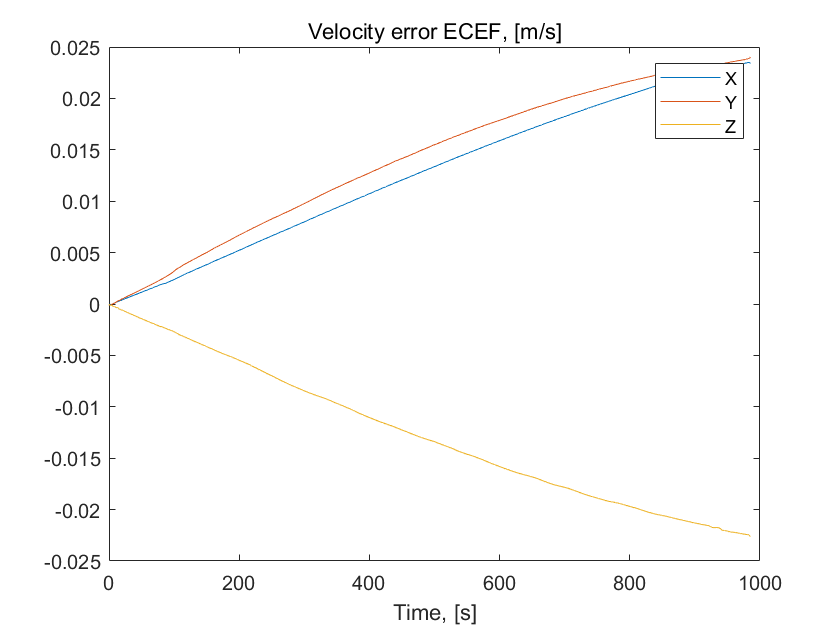
\includegraphics[width=1.0\columnwidth]{fig6.png}}
    \caption{Velocity error ECEF - 100Hz,[m/s]}
\end{figure}

\begin{figure}[htbp]
    \centerline{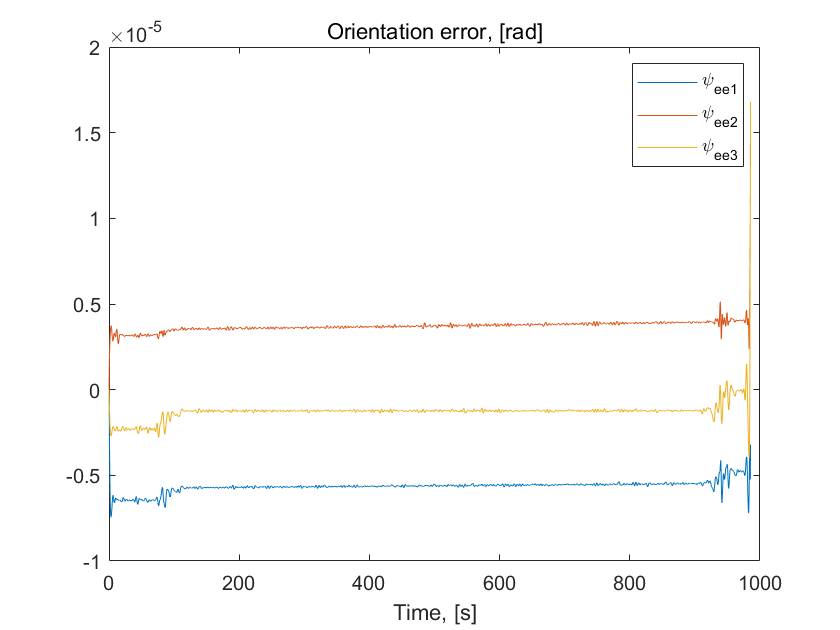
\includegraphics[width=1.0\columnwidth]{fig7.png}}
    \caption{Orientation error - 100Hz,[rad]}
\end{figure}

\begin{figure}[htbp]
    \centerline{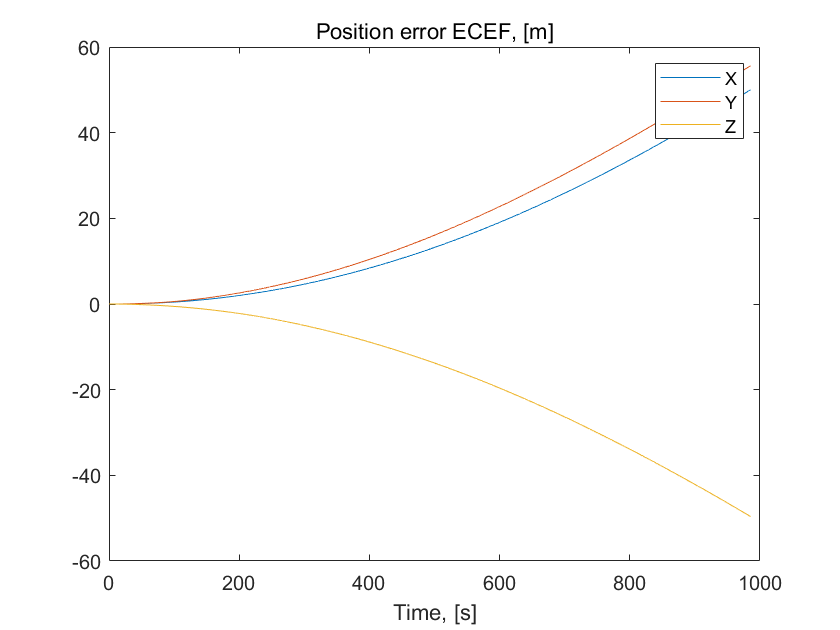
\includegraphics[width=1.0\columnwidth]{50fig1.png}}
    \caption{Position error ECEF - 50Hz}
\end{figure}

\begin{figure}[htbp]
    \centerline{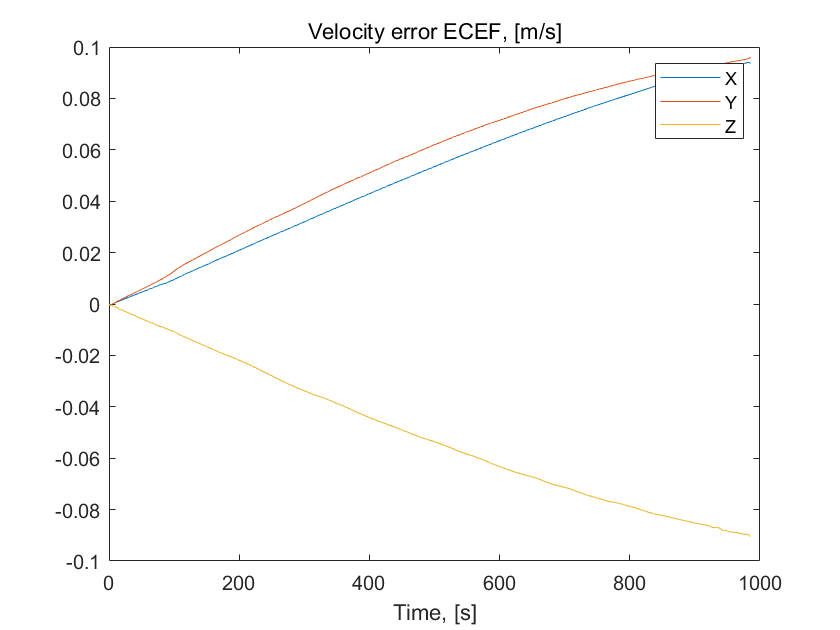
\includegraphics[width=1.0\columnwidth]{50fig2.png}}
    \caption{Velocity error ECEF - 50Hz,[m/s]}
\end{figure}

\begin{figure}[htbp]
    \centerline{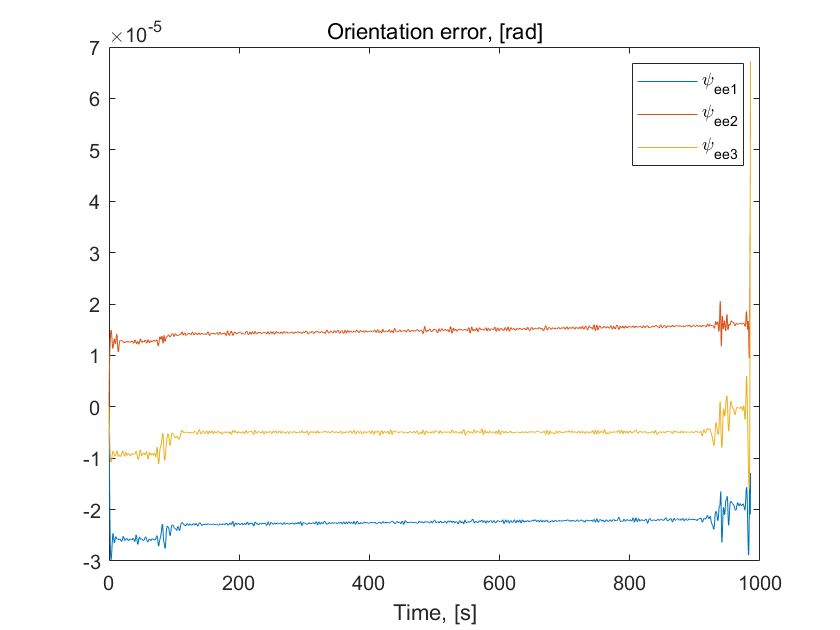
\includegraphics[width=1.0\columnwidth]{50fig3.png}}
    \caption{Orientation error - 50Hz,[rad]}
\end{figure}


\section{Loosely coupled INS/GNSS Algorithm}
In parallel to “navigating purely inertially”, it is necessary to estimate errors of position, velocity, and orientation using information from external measurement systems, such as a GNSS receiver, for example, since accuracy of the navigation parameters determined by an inertial navigation system degrades continuously due to IMU's instrumental errors, initial state errors, and errors of numerical integration. The obtained error estimates can then be used to correct position, velocity, and orientation information. In general, external measurements are not required to be available continuously, because INS is able to do dead reckoning using IMU information only. The rate of accuracy degradation during dead reckoning strongly depends on IMU accuracy class.

Figure 11 illustrates the described principles of an aided inertial navigation system.
\begin{figure}[htbp]
    \centerline{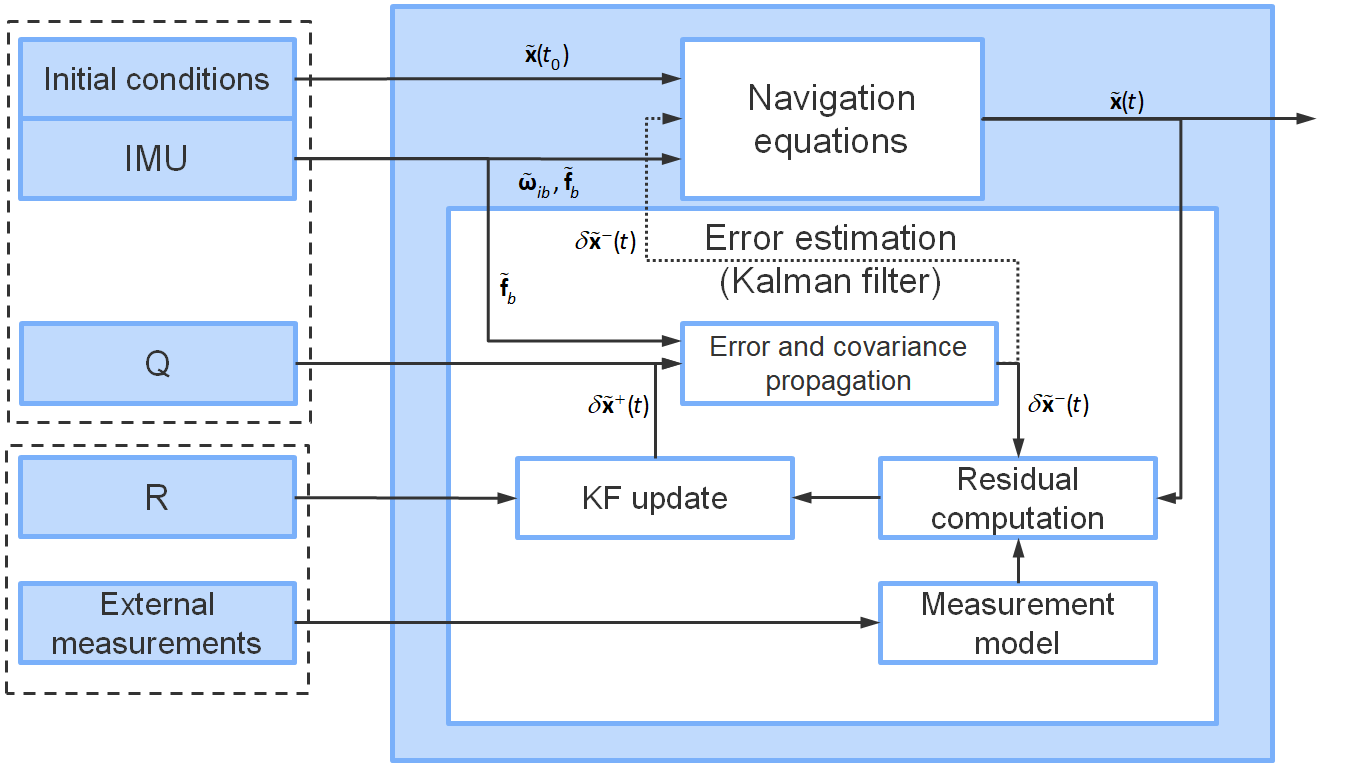
\includegraphics[width=1.0\columnwidth]{overframe.png}}
    \caption{Principles of aided inertial navigation}
\end{figure}

\subsection{Design and Architecture of the Filter}
In the navigation filter we would like to estimate sensor compensation parameters: scale factors and biases. Then, the core INS state vector needs to be augmented with the corresponding parameters. In addition to that, we will estimate alignment between the IMU frame (s-frame) and the car-fixed coordinate frame. Finally, augmented state vector will take the form:

\begin{equation}
% \begin{aligned}
z = ((X_e)^T \, (V_e)^T \, (q_{es})^T \, (b_f)^T \, (b_{\omega})^T \, (s_f)^T \, (s_{\omega})^T \, (q_cs)^T)
% \end{aligned}
\end{equation}

For dynamics of the augmented state, we will use IMU measurement compensated to propagate the state vector. Thus, the estimate of the state vector (3) is subject to:

\begin{equation}
\begin{aligned}
& \dot{\tilde{\mathbf{x}}}_e=\tilde{\mathbf{v}}_e \\
& \dot{\tilde{\mathbf{v}}}_e=-2\left[\boldsymbol{\omega}_{i e} \times\right] \tilde{\mathbf{v}}_e+\mathbf{g}_e\left(\tilde{\mathbf{x}}_e\right)+\mathbf{C}_{\tilde{e} s} \hat{\mathbf{f}}_s \\
& \dot{\mathbf{q}}_{\tilde{e} s}=\frac{1}{2}\left(\breve{\mathbf{q}}_{\tilde{e} s} * \widehat{\boldsymbol{\omega}}_{i s}-\breve{\boldsymbol{\omega}}_{i e} * \breve{\mathbf{q}}_{\tilde{e} s}\right) \\
& \hat{\mathbf{b}}_f=\mathbf{0} \\
& \hat{\mathbf{b}}_\omega=\mathbf{0} \\
& \hat{\mathbf{s}}_f=\mathbf{0} \\
& \hat{\mathbf{s}}_\omega=\mathbf{0} \\
& \dot{\mathbf{q}}_{\tilde{c} s}=\mathbf{0}
\end{aligned}
\end{equation}

For state propagation, the state vector is propagated by integrating numerically the ODE (4). Heun’s method ($2^{nd}$ order Runge-Kutta method with $\alpha = 1$) is employed. Discrete times forming the integration grid are taken from gyroscope measurements. A smartphone cannot ensure that accelerometer data and gyroscope data are collected simultaneously, so specific force needs to be interpolated or approximated at the timestamps of gyroscope measurements.

And error state vector that corresponds to the state vector (3) is given by:

\begin{equation}
% \begin{aligned}
z = ((\delta X_e)^T (\delta V_e)^T (\delta q_{es})^T (\delta b_f)^T (\delta b_{\omega})^T (\delta s_f)^T (\delta s_{\omega})^T (\delta q_cs)^T)
% \end{aligned}
\end{equation}

Dynamics of the error state is subject to linear stochastic differential equation given below. This equation can be obtained by modeling sensor errors as random walk as below:

\begin{equation}
% \begin{aligned}
\delta \dot z = A(t)*\delta z + G(t)*v
% \end{aligned}
\end{equation}
Here, the parameters are:

\begin{equation}
\tiny
\begin{aligned}
% \begin{split}
\mathbf{A}(t)=\left(\begin{array}{cccccccc}
\begin{smallmatrix}
\mathbf{0}_{3 \times 3} & \mathbf{I}_{3 \times 3} & \mathbf{0}_{3 \times 3} & \mathbf{0}_{3 \times 3} & \mathbf{0}_{3 \times 3} & \mathbf{0}_{3 \times 3} & \mathbf{0}_{3 \times 3} & \mathbf{0}_{3 \times 3} \\
\mathbf{0}_{3 \times 3} & -2\left[\boldsymbol{\omega}_{i e} \times\right] & -\left[\left(\mathbf{C}_{\tilde{e}} \hat{\mathbf{f}}_s\right) \times\right] & \mathbf{C}_{\tilde{e} s} & \mathbf{0}_{3 \times 3} & \mathbf{C}_{\tilde{e} s} \operatorname{diag}\left(\tilde{\mathbf{f}}_s\right) & \mathbf{0}_{3 \times 3} & \mathbf{0}_{3 \times 3} \\
\mathbf{0}_{3 \times 3} & \mathbf{0}_{3 \times 3} & -\left[\boldsymbol{\omega}_{i e} \times\right] & \mathbf{0}_{3 \times 3} & \mathbf{c}_{\tilde{e} s} & \mathbf{0}_{3 \times 3} & \mathbf{C}_{\tilde{e} s} \operatorname{diag}\left(\widetilde{\boldsymbol{\omega}}_{i s}\right) & \mathbf{0}_{3 \times 3} \\
\mathbf{0}_{3 \times 3} & \mathbf{0}_{3 \times 3} & \mathbf{0}_{3 \times 3} & \mathbf{0}_{3 \times 3} & \mathbf{0}_{3 \times 3} & \mathbf{0}_{3 \times 3} & \mathbf{0}_{3 \times 3} & \mathbf{0}_{3 \times 3} \\
\mathbf{0}_{3 \times 3} & \mathbf{0}_{3 \times 3} & \mathbf{0}_{3 \times 3} & \mathbf{0}_{3 \times 3} & \mathbf{0}_{3 \times 3} & \mathbf{0}_{3 \times 3} & \mathbf{0}_{3 \times 3} & \mathbf{0}_{3 \times 3} \\
\mathbf{0}_{3 \times 3} & \mathbf{0}_{3 \times 3} & \mathbf{0}_{3 \times 3} & \mathbf{0}_{3 \times 3} & \mathbf{0}_{3 \times 3} & \mathbf{0}_{3 \times 3} & \mathbf{0}_{3 \times 3} & \mathbf{0}_{3 \times 3} \\
\mathbf{0}_{3 \times 3} & \mathbf{0}_{3 \times 3} & \mathbf{0}_{3 \times 3} & \mathbf{0}_{3 \times 3} & \mathbf{0}_{3 \times 3} & \mathbf{0}_{3 \times 3} & \mathbf{0}_{3 \times 3} & \mathbf{0}_{3 \times 3} \\
\mathbf{0}_{3 \times 3} & \mathbf{0}_{3 \times 3} & \mathbf{0}_{3 \times 3} & \mathbf{0}_{3 \times 3} & \mathbf{0}_{3 \times 3} & \mathbf{0}_{3 \times 3} & \mathbf{0}_{3 \times 3} & \mathbf{0}_{3 \times 3}
\end{smallmatrix}
\end{array}\right)
% \end{split}
\end{aligned}
\end{equation}

\begin{equation}
\mathbf{G}(t)=\left(\begin{array}{ccccccc}
\mathbf{0}_{3 \times 3} & \mathbf{0}_{3 \times 3} & \mathbf{0}_{3 \times 3} & \mathbf{0}_{3 \times 3} & \mathbf{0}_{3 \times 3} & \mathbf{0}_{3 \times 3} & \mathbf{0}_{3 \times 3} \\
\mathbf{C}_{\tilde{e} s} & \mathbf{0}_{3 \times 3} & \mathbf{0}_{3 \times 3} & \mathbf{0}_{3 \times 3} & \mathbf{0}_{3 \times 3} & \mathbf{0}_{3 \times 3} & \mathbf{0}_{3 \times 3} \\
\mathbf{0}_{3 \times 3} & \mathbf{C}_{\tilde{e} s} & \mathbf{0}_{3 \times 3} & \mathbf{0}_{3 \times 3} & \mathbf{0}_{3 \times 3} & \mathbf{0}_{3 \times 3} & \mathbf{0}_{3 \times 3} \\
\mathbf{0}_{3 \times 3} & \mathbf{0}_{3 \times 3} & \mathbf{I}_{3 \times 3} & \mathbf{0}_{3 \times 3} & \mathbf{0}_{3 \times 3} & \mathbf{0}_{3 \times 3} & \mathbf{0}_{3 \times 3} \\
\mathbf{0}_{3 \times 3} & \mathbf{0}_{3 \times 3} & \mathbf{0}_{3 \times 3} & \mathbf{I}_{3 \times 3} & \mathbf{0}_{3 \times 3} & \mathbf{0}_{3 \times 3} & \mathbf{0}_{3 \times 3} \\
\mathbf{0}_{3 \times 3} & \mathbf{0}_{3 \times 3} & \mathbf{0}_{3 \times 3} & \mathbf{0}_{3 \times 3} & \mathbf{I}_{3 \times 3} & \mathbf{0}_{3 \times 3} & \mathbf{0}_{3 \times 3} \\
\mathbf{0}_{3 \times 3} & \mathbf{0}_{3 \times 3} & \mathbf{0}_{3 \times 3} & \mathbf{0}_{3 \times 3} & \mathbf{0}_{3 \times 3} & \mathbf{I}_{3 \times 3} & \mathbf{0}_{3 \times 3} \\
\mathbf{0}_{3 \times 3} & \mathbf{0}_{3 \times 3} & \mathbf{0}_{3 \times 3} & \mathbf{0}_{3 \times 3} & \mathbf{0}_{3 \times 3} & \mathbf{0}_{3 \times 3} & \mathbf{I}_{3 \times 3}
\end{array}\right)
\end{equation}

For the residual, it's defined as:

\begin{equation}
\Delta y_{pos} = \tilde{y}_{pos}-\tilde{x}_{e}=\delta{x}_{e}+\delta{y}_{pos}
\end{equation}

And the measurement matrix is defined as:

\begin{equation}
\Delta H_{pos} = \frac{\partial \Delta y_{pos}}{\partial (\delta z)^T}
\end{equation}

\subsection{Aided Navigation Outcome}

Via software written in Matlab, We can get our final outcome as below:

\begin{figure}[htbp]
    \centerline{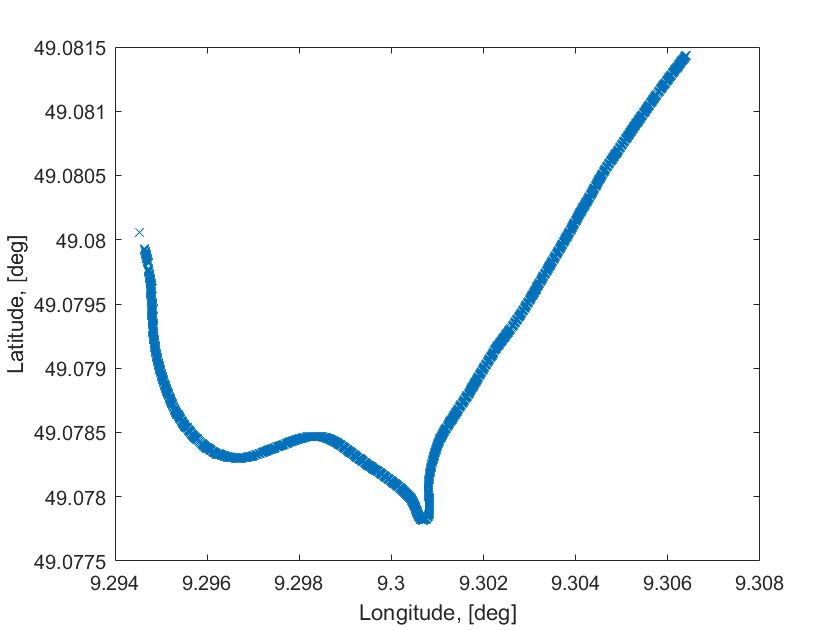
\includegraphics[width=1.0\columnwidth]{fig21.png}}
    \caption{Lat-Lon Trajectory}
\end{figure}

\begin{figure}[htbp]
    \centerline{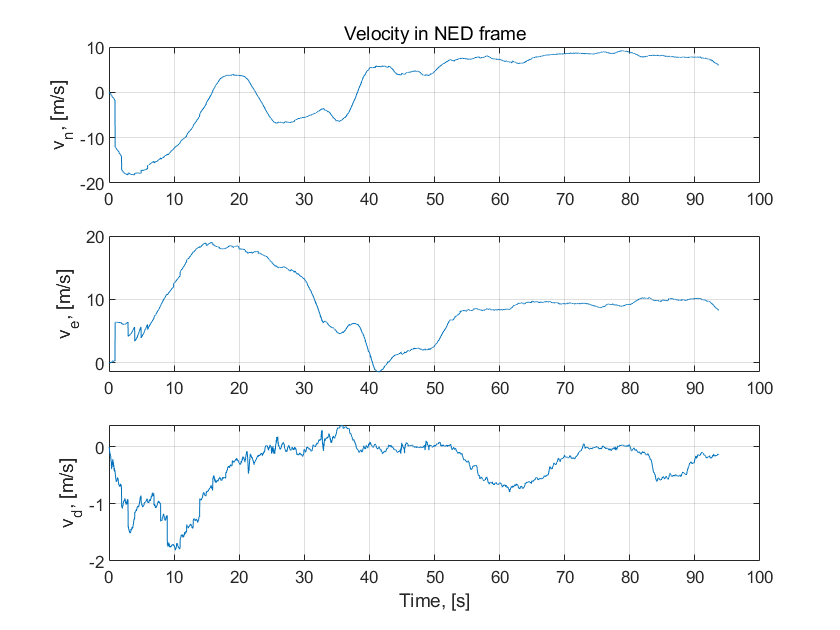
\includegraphics[width=1.0\columnwidth]{fig22.png}}
    \caption{Velocity in NED frame}
\end{figure}

\begin{figure}[htbp]
    \centerline{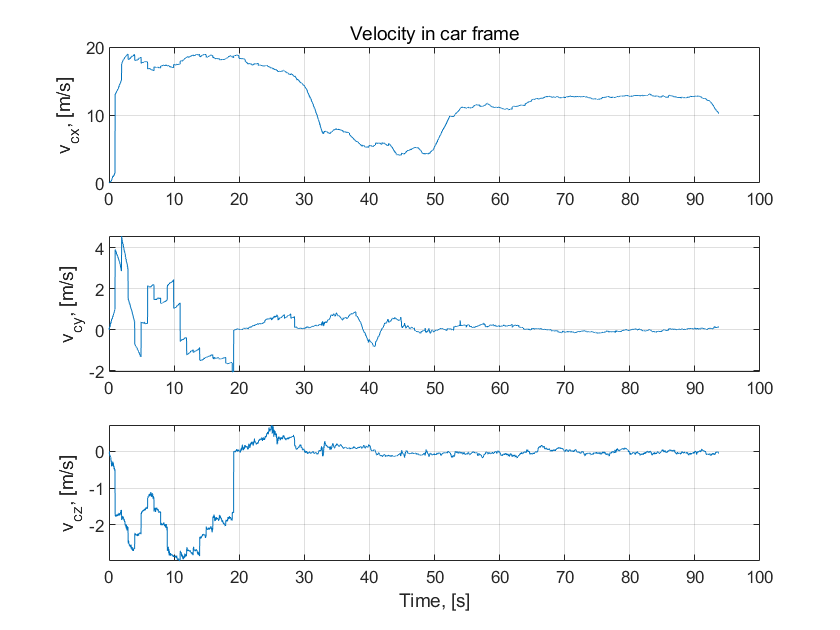
\includegraphics[width=1.0\columnwidth]{fig23.png}}
    \caption{Velocity in car frame}
\end{figure}

\begin{figure}[htbp]
    \centerline{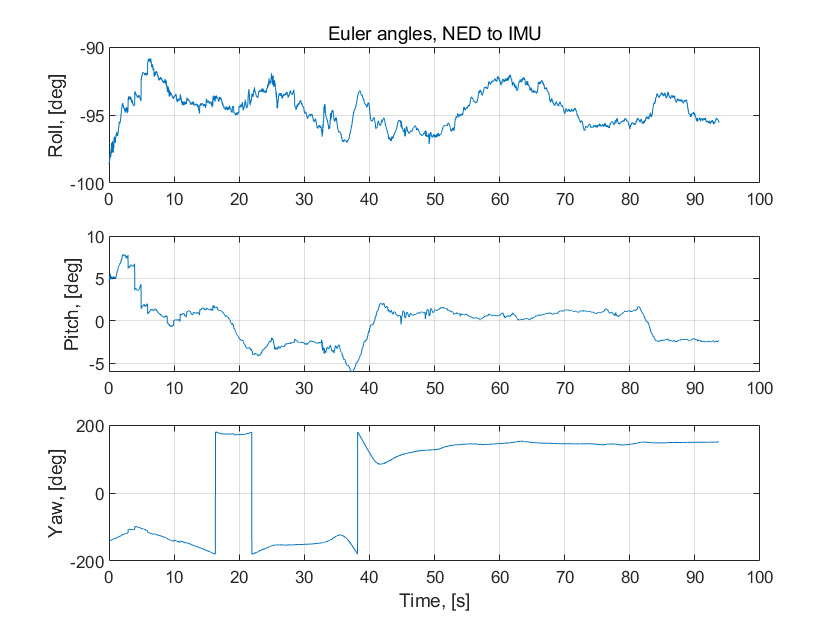
\includegraphics[width=1.0\columnwidth]{fig24.png}}
    \caption{Euler angles NED to IMU}
\end{figure}

\begin{figure}[htbp]
    \centerline{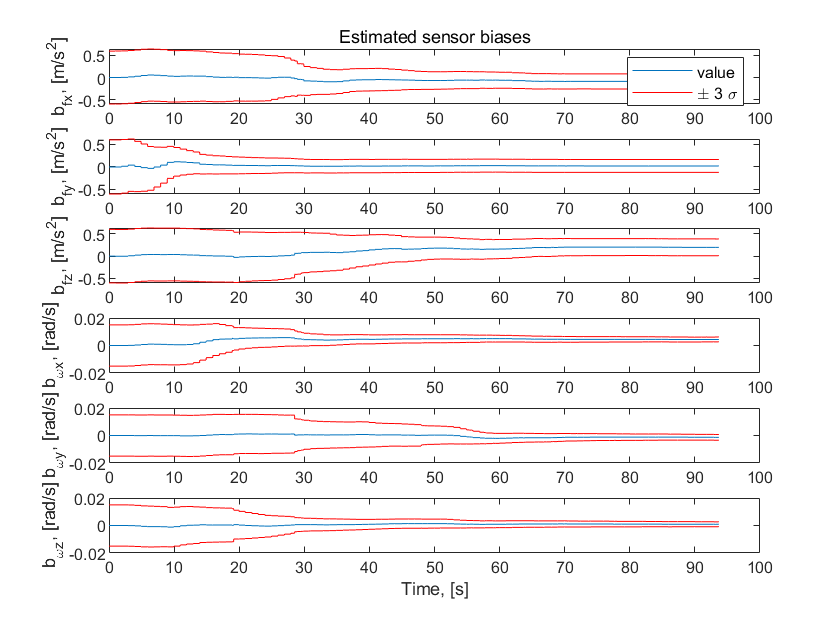
\includegraphics[width=1.0\columnwidth]{fig25.png}}
    \caption{Estimated sensor biases}
\end{figure}

\begin{figure}[htbp]
    \centerline{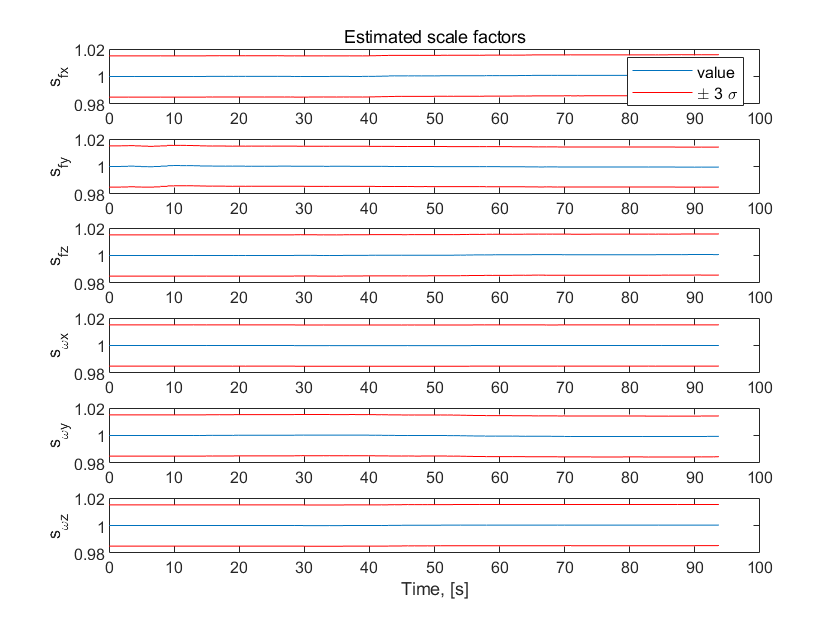
\includegraphics[width=1.0\columnwidth]{fig26.png}}
    \caption{Estimated scale factors}
\end{figure}

\begin{figure}[htbp]
    \centerline{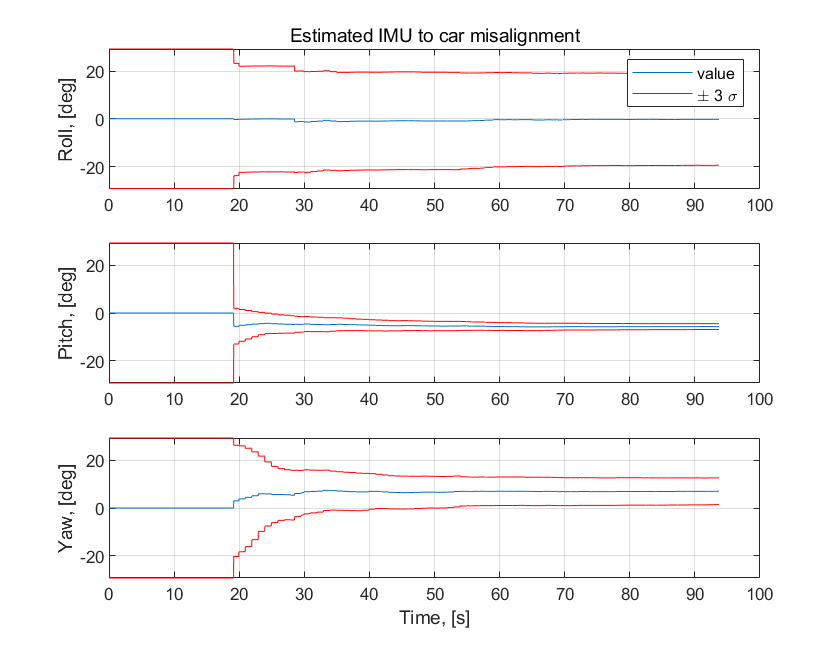
\includegraphics[width=1.0\columnwidth]{fig27.png}}
    \caption{Estimated IMU to car misalignment}
\end{figure}


\section{Configuration of ROS Platform and Visual SLAM project}

\section{Simulation Based on PX4, gazebo and ORB-SLAM2}

In this section, we use a model provided in PX4 software and equip it with stereo or mono camera,
to compose localization and mapping test in a gazebo environment provided by ROS.

\subsection{PX4 software}
The architecture of PX4 can be divided into two parts: one is the flight control stack, 
which mainly includes the flight control system and the status estimation algorithm; 
the other is the intermediate control communication layer. 
It mainly covers the driver of embedded devices, 
with external communication and UORB message bus of PX4. 
The system supports a variety of models and devices, 
but the use of a code library is used, and the design concept of "response" is used, 
which means that it can be divided into a number of functions to be divided into several. 
Demand replacement components and communication through asynchronous methods, 
such a design also allows the system to have different coping methods under different workloads. 
The following studies the flight control stack and intermediate communication layer.

\begin{figure}[htbp]
    \centerline{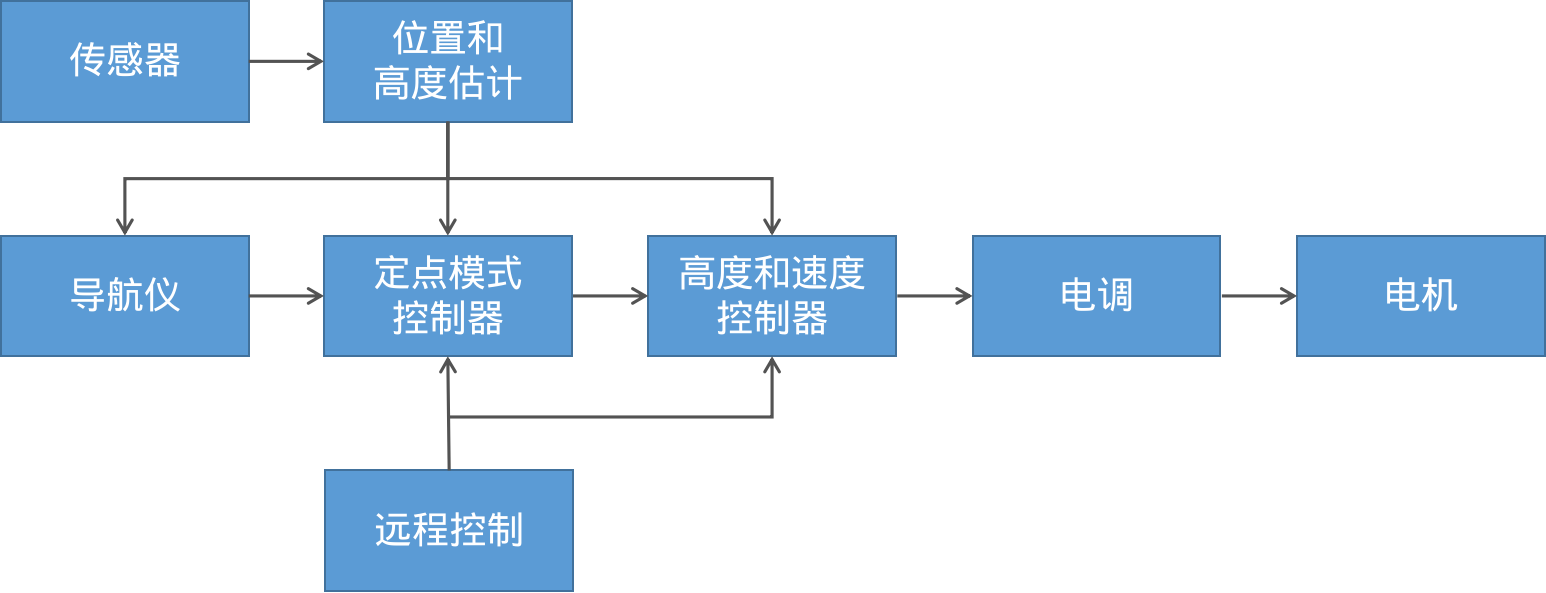
\includegraphics[width=0.95\columnwidth]{px4structure.png}}
    \caption{PX4 software structure}
\end{figure}

There is also an important component in PX4, the Fail-Safe mechanism.
That is, the safety effectiveness mechanism, 
the meaning is: when the error occurs, 
the aircraft protects or restores to a safe state to avoid the adverse consequences that 
may cause errors. 
The FailSafe system of PX4 is editable, 
which means that developers can set up a trigger on FailSafe according to their own needs to ensure experiments or complete tasks under security. 
After the FailSafe system is triggered, there are generally several feedback measures for automatic landing, 
keeping the location or returning specific routes.

Generally, ECL and EKF will appear at the same time. 
ECL is the estimation and control Library, status estimation and control library; 
EKF is Extended Kalman Filter. 
Expanding Carman filtering is an optimized algorithm. 
The combination of the two is the state of estimation and control library using the extended Karman filtering method. 
Its role is the data of the processing sensor, 
and the speed and position of the processing of the IMU (inertia measurement unit), 
the rotation matrix, wind speed and wind speed and wind speed of the quad -dollar number, 
Machining and estimation of information obtained by the magnetic compass is processed and estimated. 
EKF uses IMU, magnetic meter, height meter, GPS, speed meter and other sensors. 
In order to change the height and position of the traditional air pressure meter+GPS to the height 
and position estimation of the visual information, 
the relevant parameters of the EKF sensor need to be modified. 

\subsection{Mavros Velocity Control Method}
Although the Position information can be controlled by the Office point in the offboard mode, 
the actions of drone take off and move forward are too large, 
which directly affects the tracking effect of the SLAM system. 
Therefore, 
it is necessary to consider the information posted through Mavros to control the speed of the drone.

\begin{figure}[htbp]
    \centerline{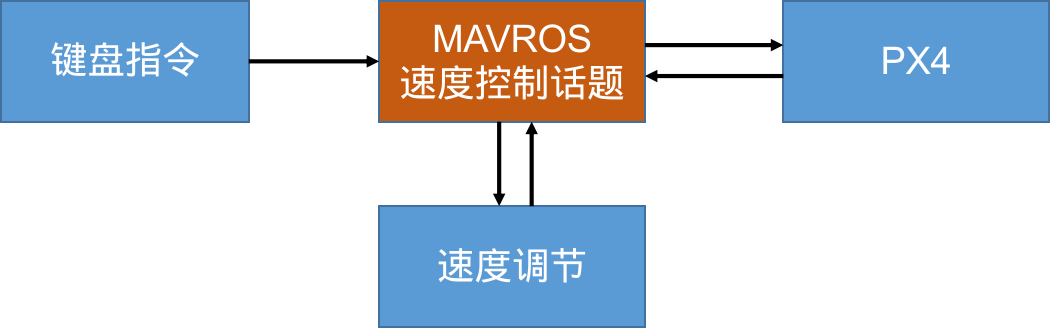
\includegraphics[width=0.8\columnwidth]{keyboard.png}}
    \caption{Mavros Velocity Control}
\end{figure}

Table tab-mavros shows a command of keyboard control to mavros topics.

\begin{table}[htbp]
    \caption{Command of keyboard}
    \label{tab-mavros}
\begin{center}
    \begin{tabular}{cc}
        \hline
        Key& Function\\
        \hline
		W& add velocity in x axis\\
		S& decrease velocity in x axis\\
		A& add velocity in y axis\\
		D& decrease velocity in y axis\\
		
		Page Up    & add velocity in z axis\\
		Page Down  & decrease velocity in z axis\\
		Page Left  & add rotate velocity in z axis\\
		Page Right & decrease rotate velocity in z axis\\
		
		T & offboard and takeoff\\
		L & landing mode\\
		H & hold position\\
        \hline
    \end{tabular}
\end{center}
\end{table}

\subsection{Visual SLAM, ORB-SLAM2 example}

In various SLAMs, the visual SLAM has become the most commonly used way in SLAM due to the low cost of its sensor (optical camera). 
It is necessary to understand the principle of using the visual SLAM of the camera. 
First of all, you need to understand the imaging principle and parameters of the camera.

\begin{figure}[htbp]
    \centerline{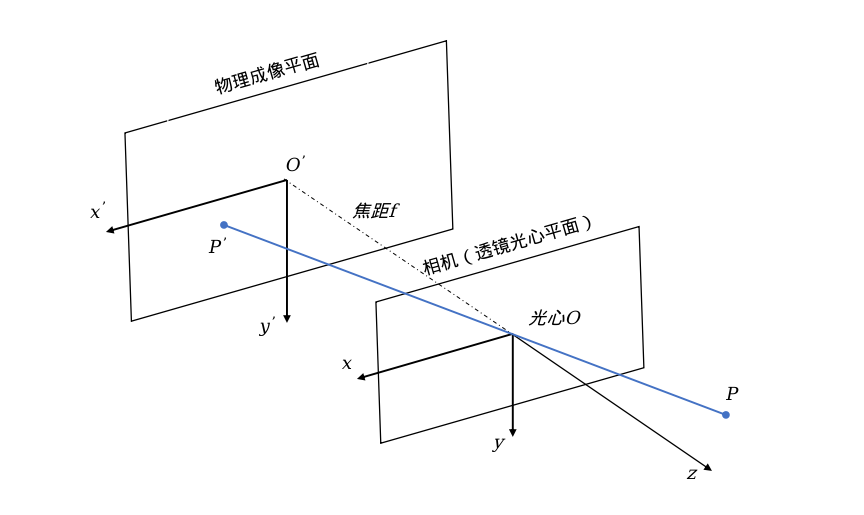
\includegraphics[width=0.9\columnwidth]{camera.png}}
    \caption{camera model}
\end{figure}

After the small hole O projection, the coordinate of the camera coordinate system on the pixel plane is
Under theory, small holes are imagined as an inverted image, but in the actual camera, 
the imaging is artificially rotated and established. 
Therefore, the impact of the positive number of the coordinate system is not considered.

\begin{equation}
    \frac{Z}{f}=\frac{X}{X'}=\frac{Y}{Y'}
\end{equation}

On this basis, define the pixel coordinate system. 
The pixel coordinate system is a two -dimensional coordinate system, 
which is on the plane of physical imaging. 
The original point of the pixel coordinate system is located in the upper left corner of the image. 
The horizontal axis is a U -axis. The right is parallel to the X axis. 
The relationship between pixel coordinates and P' coordinates can be obtained:

\begin{equation}
    \begin{cases}
    u=\alpha X'+c_x=\alpha f \cfrac{X}{Z}+c_x \\
    v=\beta Y' +c_y=\beta f  \cfrac{Y}{Z}+c_y \\
    \end{cases}
\end{equation}

Convert the coordinates under the pixel coordinate system to Qi Angle coordinates: 

\begin{equation}
    \begin{bmatrix}
    u\\v\\1
    \end{bmatrix}=
    \frac{1}{Z}
    \begin{bmatrix}
    f_x & 0 & c_x\\
    0   & f_y & c_y\\
    0 & 0 & 1
    \end{bmatrix}
    \begin{bmatrix}
    X\\Y\\Z
    \end{bmatrix}=
    \frac{1}{Z} \bf{KP}
    \end{equation}

The Camera Intrinsics K was obtained. 
Under normal circumstances, 
for the camera (or fixed focus lens) with focal length fixation, 
the end-clicpice matrix is fixed after the factory. 
If the internal reference of the camera cannot be obtained from the manufacturer, 
the calibration method can be used to obtain the internal reference matrix of the camera. 
The common calibration algorithm is the Zhang Zhengyou calibration method.

In addition to the internal parameters of the camera, 
there is also the definition of Camera Extrinsics. 
The external parameter of the camera consists of its rotating matrix R peace move vector T. 
For point P, 
the coordinates under the camera coordinate system (pixel coordinate plane) shall be transformed 
by its coordinates under the world coordinate system according to the camera compared to the world 
coordinate system. The position of the camera is determined by its external parameters, 
and the coordinate of the coordinate PW of Point PW under the world coordinate system is:

\begin{equation}
    Z
    \begin{bmatrix}
    u\\v\\1
    \end{bmatrix}=
    \bf{K(RP_w+t)}
\end{equation}

The purpose of the tracking thread is to obtain the current position of the camera from each frame observed by the camera; 
in the process, according to the feature points of the local map, only use the motion estimate BA to minimize the heavy projection error. 
First enter the pre -processing phase of the current frame. 
In this part, the ORB feature point extraction and matching link of the current frame will be completed, 
and the key points of the requirements are finally met. 
The estimation of the current camera position and connect with the local map to get the tracking in the map, 
and finally decide whether the frame can be inserted into a key frame database as a key frame.

\begin{figure}[htbp]
    \centerline{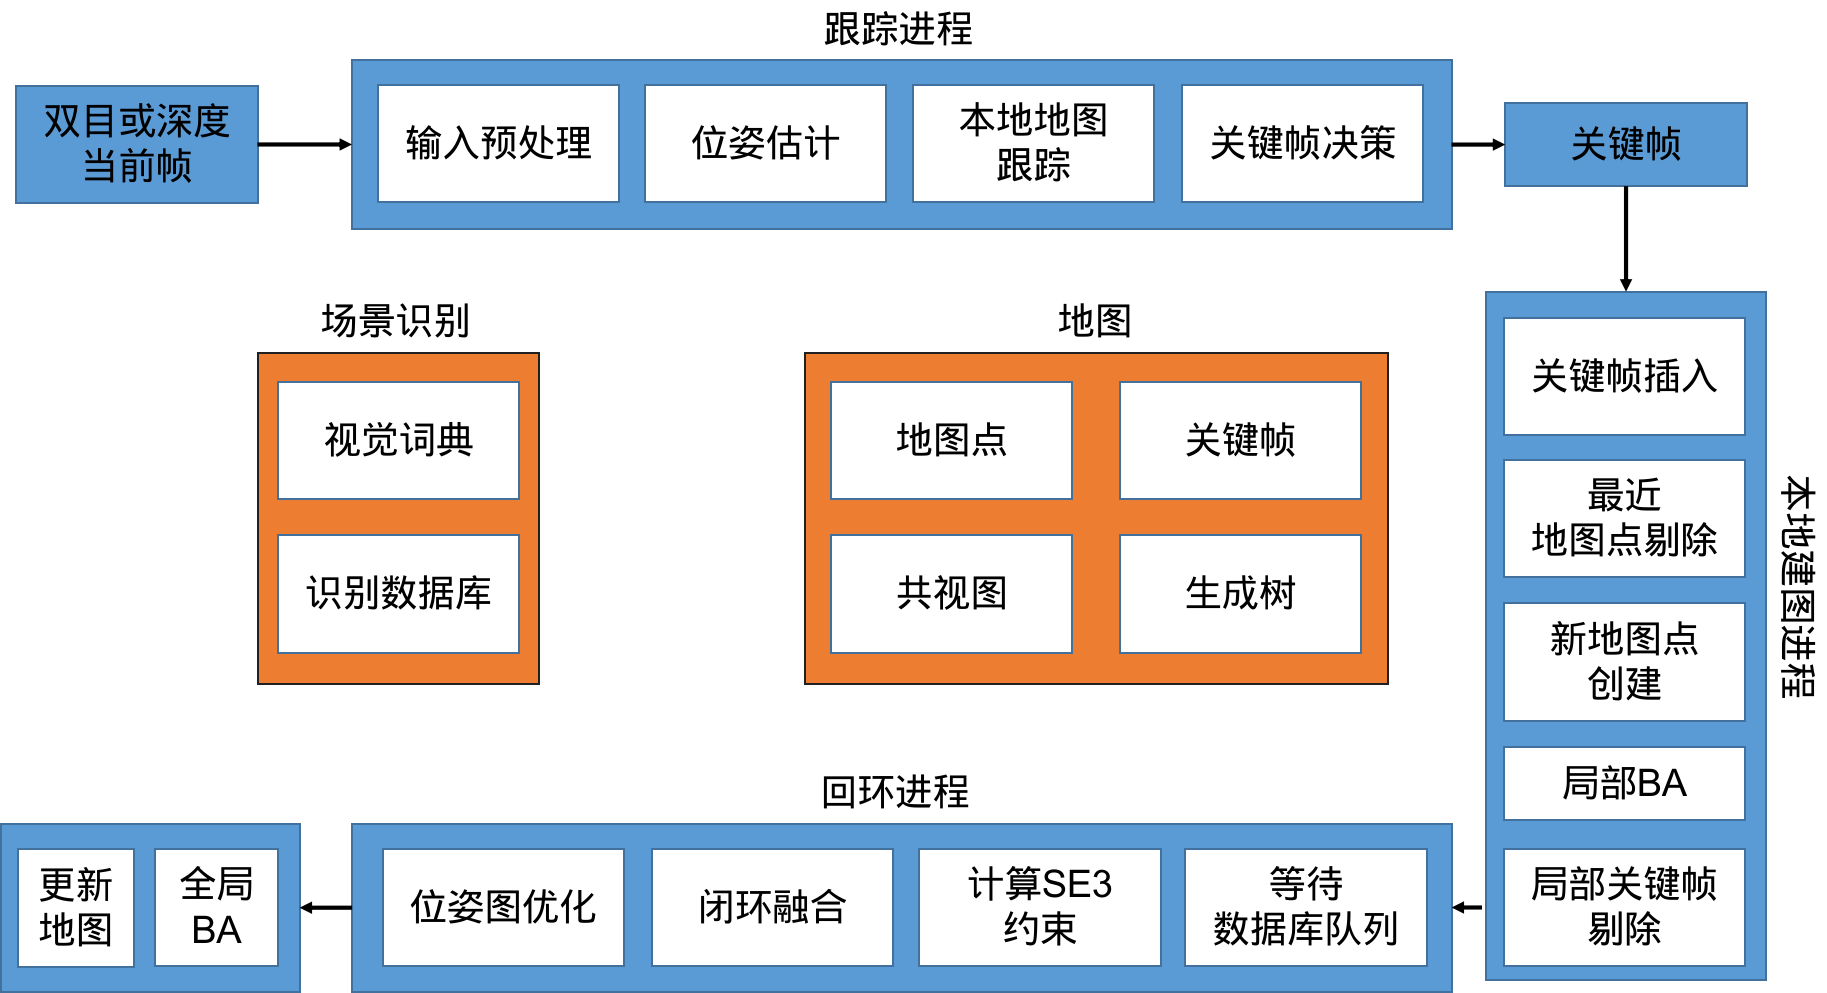
\includegraphics[width=0.9\columnwidth]{ORBstructure.png}}
    \caption{Structure of ORB-SLAM2}
\end{figure}

The purpose of building a local map is to manage local maps and perform local BAs to optimize. 
There are three BAs throughout ORB-SLAM. First, the sports model BA in the tracking thread, 
the other is to optimize the local BA of key frames and map points in the local map, 
and the global BA after the final return to the loop detection. These are the G2O -based LM trust. 
Domain convergence optimization method. In this thread, the content of the input is a key frame. 
First of all, 
the insertion of the key frame must be completed. Remove some key frames.

The purpose of the loop -loop thread is to complete the loop return detection and optimize the cumulative error through the position map; 
after the closed loop is detected and the merger is completed, 
the global BA thread will be opened to optimize the global path. 
After experiencing a local planning thread, the key frame will enter the loop thread; 
the first is to return the loop detection. In this case, the SE3 calculation is required. 
It requires not only to meet the similar relationship, 
but also the key frames that meet the geometric constraints to enter the closed loop of the ring ring. 
During the correction; when entering the correction phase, after the closed loop is fused, the position is optimized. 
After that, start a new global optimization process,
 carry out global BA optimization, and update the optimized map.

\subsection{gazebo scene simulation}

It can be seen that after a whole circle of flight, 
the SLAM system has successfully detected the return loop and completed the cumulative error elimination 
and the optimization of the overall map.

\begin{figure}[htbp]
    \centerline{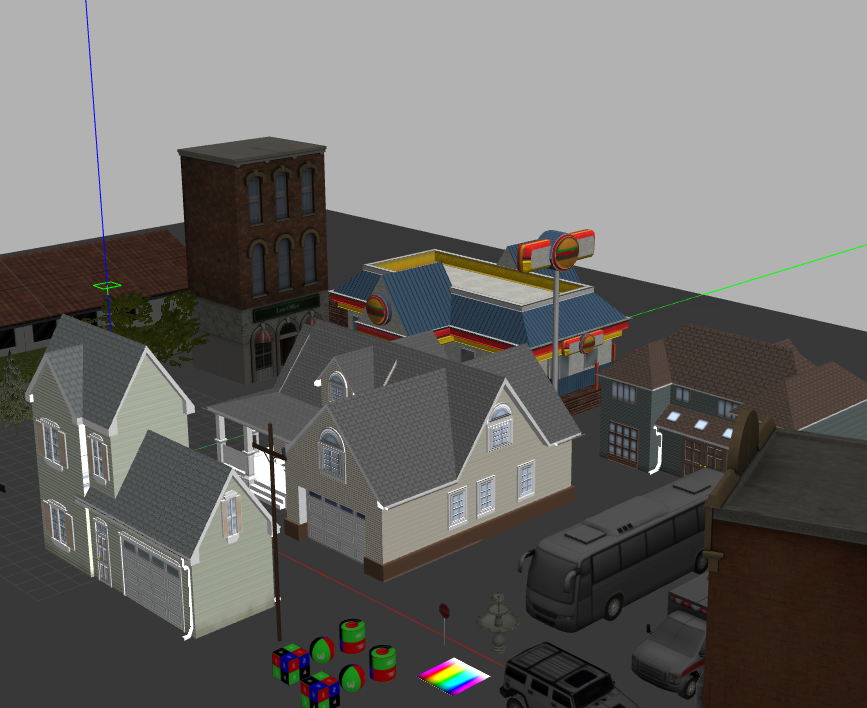
\includegraphics[width=0.9\columnwidth]{stereo1.png}}
    \caption{gazebo scene}
\end{figure}

We create a scene that easy to complete the loop fusion procedure.

\begin{figure}[htbp]
    \centerline{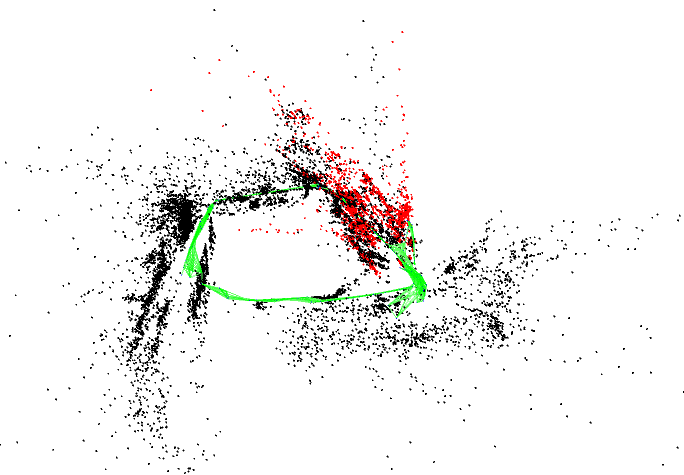
\includegraphics[width=0.9\columnwidth]{stereo3.png}}
    \caption{gazebo scene}
\end{figure}

\subsection{Euroc Dataset test}

After that, we use datasets of ASL to test the ORB-SLAM2.

EVO is a trajectory developed by SLAM's visualization and position analysis software developed by Michael Grupp. 
It supports TUM, EUROC, Kitti data set format, and can be converted to each other; 
SIM3 conversion, after obtaining alignment, 
the position is true and the visual trajectory is compared; 
and the absolute error can be analyzed, the accuracy of the judgment of the algorithm

\begin{figure}[htbp]
    \centerline{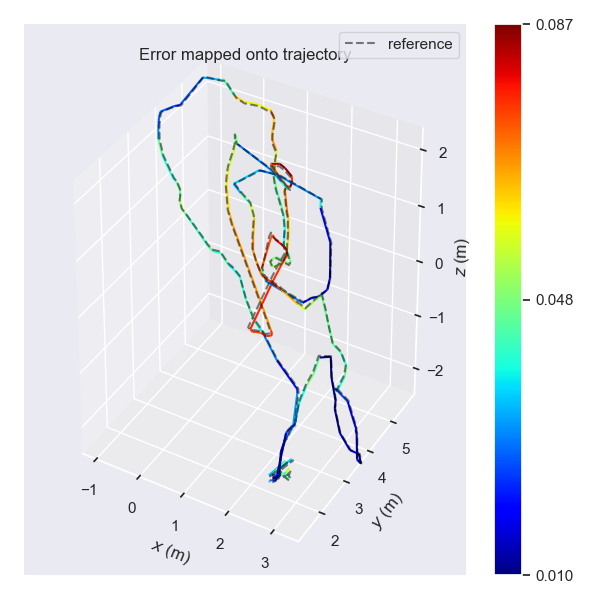
\includegraphics[width=0.9\columnwidth]{ape_map0.png}}
    \caption{ground truth and SLAM result}
\end{figure}

It can be seen that the SLAM result is rather close to the ground truth.


\section{Conclusion}

The project aims to realize and explain state of the art methods of modern aided navigation and multi-sensor localization.

Via software written in Matlab, We realize a loosely-coupled fusion INS/GNSS sensor system and plot the Lat-Lon trajectory.

After that, via the simulation data generated from software, we simulates ideal IMU measurements at different frequency, the code outcome serving as an evidence of IMU data being “ideal” as well. 

We also use ORB-SLAM2 to run simulation in a street scene and in Euroc datasets, the results are satisfied.

However, due to limit of time, we didn't combine visual information, IMU data and GNSS location together, with only individual completion.

% \nocite{*}
% \bibliographystyle{IEEEtran}
% \bibliography{IEEEabrv,bmy}

\begin{thebibliography}{00}
\bibitem{b1} Jazwinski, A. H. (2007). Stochastic Processes and Filtering Theory. Mineola, New York: Dover Publications, Inc.Phil. Trans. Roy. Soc. London, vol. A247, pp. 529--551, April 1955.
\bibitem{b2} Baklanov, F. (2017). Platform-autonomous Fault-tolerant Attitude/Heading Reference and Navigation Systems. München: Technische Universität München.
\bibitem{b3} Farrell, J. (2008). Aided Navigation: GPS with High Rate Sensors. McGraw-Hill.
\bibitem{b4} Grewal, M. S. (2014). Kalman Filtering: Theory and Practice with MATLAB. Wiley-IEEE Press.
\bibitem{b5} fedorbaklanov , (2022)[open-aided-navigation].https://github.com/fedorba \\
klanov/open-aided-navigation
\end{thebibliography}
\vspace{12pt}

\end{document}
